\documentclass[twocolumn]{article}

\usepackage[margin=0.5in]{geometry}
\usepackage{amsmath}
\usepackage{tikz}

\title{2.4 More Combinatorics Notes}
\author{}
\date{}

\begin{document}
\maketitle

\section*{Concepts}

\subsection*{Paths on a Grid}
Combinations sometimes appear in places where you don't expect them.
One example of this is counting the number of paths on a grid.
Let's say we have a $4$ by $5$ grid and we wanted to know the number of paths from the top left corner to the bottom right corner which only move downwards and rightwards.
\begin{center}
	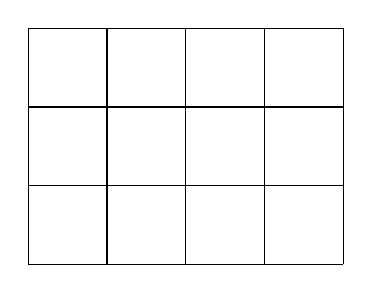
\begin{tikzpicture}
		\draw (0,0) grid (4,3);
	\end{tikzpicture}
\end{center}In order to get from the top left corner to the bottom right corner, we have to move downwards exactly three times and move rightwards exactly four times in any order.
We make seven moves in total and we can choose three of them to be downwards moves, so there are $\binom{7}{3} = \frac{7 \cdot 6 \cdot 5}{3 \cdot 2} = 35$ paths satisfying the restrictions.

\subsection*{Complementary Counting}
If we want to count the number of objects satisfying a certain property, it is often easier to count the number of objects which do not satisfy the property and then subtract it from the total.
You should try complementary counting before going into tedious casework.

To demonstrate complementary counting, we can look at problem 21 from the 2006 AMC 10A.
It asks to count the number of \textbf{four-digit positive integers} that have \textbf{at least} one digit that is a $2$ or a $3$.
First of all, notice that four-digit positive integers are not the same as four-digit sequences, because the first digit can't be $0$.
If we tried to count the number of possibilities for each digit, we will quickly run into a problem: the possible values for one digit depends on the values of the other digits.
If the first digit is $2$ or $3$, then the other digits can be anything, but if the first digit is not $2$ or $3$, then the other digits must have a $2$ or $3$.
We can go through all the cases, but there's a better way.
We first count the number of four-digit positive integers which don't have a $2$ or a $3$.
This is easier to do because now the possible values of each digit don't depend on the values of other digits.
We simply can't have $2$ or $3$.
The first digit has $7$ possibilities since we exclude $0$, $2$, and $3$.
The other three digits each have $8$ possibilities, for a total of $3584$.
There are $9000$ four-digit positive integers, so the number of positive four-digit integers which have at least one $2$ or $3$ is $9000 - 3584 = 5416$.

\subsection*{Stars and Bars}
Another non-obvious application of combinations is to count the number of ways to distribute $n$ indistinguishable objects into $k$ distinguishable bins, such that no bin is empty.
To solve this problem, we can think of it as inserting $k - 1$ dividers (represented by bars) between the $n$ objects (represented by stars).
The stars to the left of the first bar are in the first bin, the stars between the first and second bars are in the second bin, and so on.
We can't put a bar to the left of the first star, to the right of the last star, or right next to another bar, because that would represent an empty bin.
Therefore there are $n - 1$ gaps between the stars where we have to place $k - 1$ bars, so the number of ways to distribute $n$ indistinguishable objects into $k$ distinguishable boxes such that no bin is empty is $\binom{n - 1}{k - 1}$.

We can also count the number of ways to distribute $n$ indistinguishable objects into $k$ distinguishable bins where a bin can be empty.
We can reduce this to the previous problem simply by adding $k$ stars.
There's a one-to-one correspondence between distributions of $n$ objects into $k$ potentially empty bins and distributions of $n + k$ objects into $k$ non-empty bins because for each distribution of the first kind, we can add an object to every bin to get a distribution of the second kind, and for each distribution of the second kind, we can remove an object from every bin to get a distribution of the first kind.
Therefore, the number of ways to distribute $n$ indistinguishable objects into $k$ distinguishable bins where a bin can be empty is $\binom{n + k - 1}{k - 1}$.

\subsection*{$\mathbf{\binom{n}{k} = \binom{n}{n - k}}$}
This is one of the most basic properties of combinations.
This is true because choosing a set of $k$ objects out of $n$ objects is the same as choosing $n - k$ objects out of $n$ objects to exclude from the set.
We can also prove this using the formula for combinations: $\binom{n}{k} = \frac{n!}{k!(n - k)!} = \frac{n!}{(n - (n - k))!(n - k)!} = \frac{n!}{(n - k)!(n - (n - k))!} = \binom{n}{n - k}$.
If you wanted to compute $\binom{100}{98}$, you can instead compute $\binom{100}{2}$, which is a little easier to think about.

\end{document}
